\begin{wrapfigure}[3]{l}{0.1\textwidth}
	\vspace{-10pt}
	
\includegraphics[width=\linewidth]{images/ikony_deja-dup.png}
\end{wrapfigure}

Program \textcolor{ubuntu_orange}{Déjà Dup} jest prostym narzędziem do robienia kopii zapasowej danych. Nie służy on do kompleksowego zarzadzania kopiami całego systemu (np. zainstalowanymi programami). Déjà Dup najbardziej się przydaje do tworzenia kopii bezpieczeństwa plików z katalogu domowego użytkownika. Na poniższym przykładzie pokazane zostanie jak stworzyć i zarządzać kopią zapasową całego katalogu domowego.

\begin{center}
	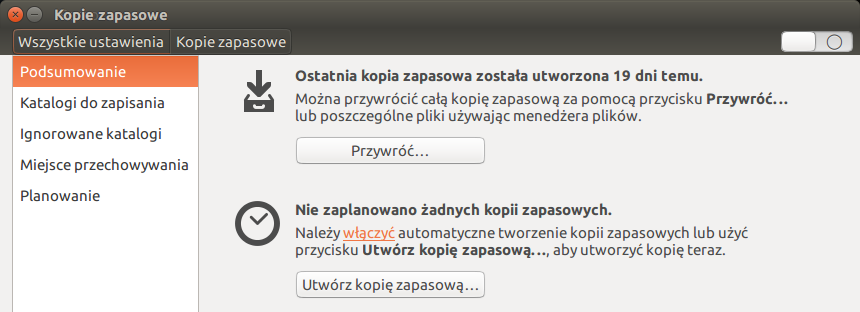
\includegraphics[width=\linewidth]{images/programy_dejavu1.png}
\end{center}

\subsubsection{Konfigurowanie kopii zapasowych}
Po pierwsze, należy uruchomić program Déjà Dup. Aby to zrobić, wpisz w Dashu \textcolor{ubuntu_orange}{Kopie zapasowe} lub w menu systemowym 
\includegraphics{images/ikony_zasilanie.png} wybierz \menu{{Ustawienia systemu\ldots}>{Kopie zapasowe}}.

W uruchomionym programie masz do wyboru 5 zakładek. Pierwsza z nich, \textcolor{ubuntu_orange}{Podsumowanie}, na razie nie jest pomocna, gdyż jeszcze nie skonfigurowałeś programu. Przejdź do \textcolor{ubuntu_orange}{Katalogów do zapisania}. Tutaj możesz wskazać, które katalogi mają być zachowywane. Domyślnie program skanuje cały katalog domowy użytkownika. Masz teraz dwie możliwości: skasować ten wpis (przycisk \textcolor{ubuntu_orange}{-} na dolnej belce), a~następnie ręcznie wskazać tylko te katalogi, które chcesz zachowywać, albo pozostawić skanowanie całego katalogu domowego i wykluczyć tylko te katalogi, których na pewno nie chcesz zachowywać. Drugie rozwiązanie jest lepsze, gdyż nie pominiesz niczego istotnego. Łatwiej jest wykluczyć kilka katalogów, niż pamiętać o włączeniu kilkuset.

Jeżeli chcesz dodać jakiś katalog, naciśnij przycisk \textcolor{ubuntu_orange}{+} i wskaż katalog spoza swojego katalogu domowego.

Zakładka \textcolor{ubuntu_orange}{Ignorowane katalogi} służy do określenia, które katalogi nie będą zapisywane. Domyślnie pomijane są katalogi kosza oraz z plikami pobranymi z internetu {Pobrane). Warto wykluczyć te, które zajmowałyby bardzo dużo miejsca. Filmy, czy gry bardzo źle się kompresują i są bardzo duże. Nie warto ich przechowywać, chyba że cierpisz na nadmiar miejsca i mocy obliczeniowej.
\begin{itemize}
\item \textcolor{ubuntu_orange}{\textasciitilde /Filmy} --- główny katalog z filmami.
\item \textcolor{ubuntu_orange}{\textasciitilde /.wine*} --- wszystkie katalogi programu Wine.
\item \textcolor{ubuntu_orange}{\textasciitilde /.local/share/Steam} --- katalog programu Steam.
\end{itemize}

\textcolor{ubuntu_orange}{Miejsce przechowywania} wskazuje, gdzie mają być zapisywane pliki z kopiami zapasowymi.  Domyślnie w katalogu domowym zostanie utworzony katalog \textcolor{ubuntu_orange}{deja-dup}, w którym będą przechowywane te pliki. Nie jest to najlepsze rozwiązanie. Podstawowa zasada tworzenia kopii zapasowych brzmi: \emph{Nie należy przechowywać kopii zapasowej na tym samym nośniku co oryginalne pliki}. Alternatywne rozwiązania to:
\begin{itemize}
\item wkazanie zamontowanego pendrive'a lub innego, zewnętrznego dysku;
\item wskazanie katalogu, z którego dane są wysyłane do chmury (np. DropBox, Copy);
\item wskazanie udziału sieciowego, aby dane były przenoszone na inny komputer.
\end{itemize}

\textcolor{ubuntu_orange}{Planowanie} pozwala ustalić kiedy, i z jaką częstotliwością, mają być wykonywane kopie zapasowe.

Teraz możesz wrócić do zakładki \textcolor{ubuntu_orange}{Podsumowanie}. Kliknij \textcolor{ubuntu_orange}{Utwórz kopię zapasową}. W otwartym oknie możesz wybrać, czy archiwum zostanie zaszyfrowane, czy nie. Jeżeli przechowujesz kopie zapasowe na innym komputerze (np. w chmurze), to warto je zaszyfrować. Utwórz hasło i kliknij \textcolor{ubuntu_orange}{Kontynuj}.

Aby włączyć automatyczne tworzenie kopii zapasowych, upewnij się, że przełącznik w prawym górnym rogu okna jest ustawiony na pozycji \textcolor{ubuntu_orange}{Włączony}.

\subsubsection{Przywracanie z backupu}
Aby przywrócić pojedyńczy plik do jego poprzedniego stanu wystarczy kliknąć go prawym przyciskiem myszy i wybrać \textcolor{ubuntu_orange}{Przywróć do poprzedniej wersji\ldots}. W otwartym oknie będziesz mieć możliwość wskazania, która wersja pliku ma zostać przywrócona.

Istnieje też możliwość przywrócenia całej utworzonej kopii zapasowej. Uruchom program \textcolor{ubuntu_orange}{Kope zapasowe} i wybierz \textcolor{ubuntu_orange}{Przywróć}. Będziesz mógł wybrać, czy wypakować pliki do pojedynczego katalogu, czy nadpisać aktualny stan twojego katalogu domowego. W drugim przypadku większość zmian wejdzie w życie dopiero po ponownym zalogowaniu do systemu.
